\documentclass{report}
\usepackage[T1]{fontenc}
\usepackage{color}
\usepackage{amssymb}
\usepackage{amsmath}
\usepackage{eurosym}
\usepackage{graphicx}
\usepackage{textcomp}
\usepackage{listings}
\usepackage{epigraph}
\usepackage{longtable}
\usepackage{setspace}
\usepackage[some]{background}
\usepackage{gensymb}
\usepackage{tikz}
\usepackage{fancyhdr}
\usepackage[margin=0.7in]{geometry}
\usepackage{tabularx}
\usepackage[english]{babel}
\definecolor{lightgray}{rgb}{0.95, 0.95, 0.95}
\definecolor{darkgray}{rgb}{0.4, 0.4, 0.4}
\definecolor{editorGray}{rgb}{0.95, 0.95, 0.95}
\definecolor{editorOcher}{rgb}{1, 0.5, 0}
\definecolor{editorGreen}{rgb}{0, 0.5, 0} 
\definecolor{orange}{rgb}{1,0.45,0.13}      
\definecolor{olive}{rgb}{0.17,0.59,0.20}
\definecolor{brown}{rgb}{0.69,0.31,0.31}
\definecolor{purple}{rgb}{0.38,0.18,0.81}
\definecolor{lightblue}{rgb}{0.1,0.57,0.7}
\definecolor{lightred}{rgb}{1,0.4,0.5}

\lstdefinelanguage{CSS}{
  keywords={color,background-image:,margin,padding,font,weight,display,position,top,left,right,bottom,list,style,border,size,white,space,min,width, transition:, transform:, transition-property, transition-duration, transition-timing-function}, 
  sensitive=true,
  morecomment=[l]{//},
  morecomment=[s]{/*}{*/},
  morestring=[b]',
  morestring=[b]",
  alsoletter={:},
  alsodigit={-}
}

\lstdefinelanguage{JavaScript}{
  morekeywords={typeof, new, true, false, catch, function, return, null, catch, switch, var, if, in, while, do, else, case, break},
  morecomment=[s]{/*}{*/},
  morecomment=[l]//,
  morestring=[b]",
  morestring=[b]'
}

\lstdefinelanguage{HTML5}{
  language=html,
  sensitive=true,   
  alsoletter={<>=-},    
  morecomment=[s]{<!-}{-->},
  tag=[s],
  otherkeywords={
  >,
    <!DOCTYPE,
  </html, <html, <head, <title, </title, <style, </style, <link, </head, <meta, />,
    </body, <body,
    </div, <div, </div>, 
    </p, <p, </p>,
    </script, <script,
  <canvas, /canvas>, <svg, <rect, <animateTransform, </rect>, </svg>, <video, <source, <iframe, </iframe>, </video>, <image, </image>, <header, </header, <article, </article
  },
  ndkeywords={
  =,
  charset=, src=, id=, width=, height=, style=, type=, rel=, href=,
  fill=, attributeName=, begin=, dur=, from=, to=, poster=, controls=, x=, y=, repeatCount=, xlink:href=,
  margin:, padding:, background-image:, border:, top:, left:, position:, width:, height:, margin-top:, margin-bottom:, font-size:, line-height:,
  transform:, -moz-transform:, -webkit-transform:,
  animation:, -webkit-animation:,
  transition:,  transition-duration:, transition-property:, transition-timing-function:,
  }
}

\lstdefinelanguage{htmlcssjs} {
  basicstyle={\footnotesize\ttfamily},   
  frame=b,
  xleftmargin={0.75cm},
  numbers=left,
  stepnumber=1,
  firstnumber=1,
  numberfirstline=true, 
  identifierstyle=\color{black},
  keywordstyle=\color{blue}\bfseries,
  ndkeywordstyle=\color{editorGreen}\bfseries,
  stringstyle=\color{editorOcher}\ttfamily,
  commentstyle=\color{brown}\ttfamily,
  language=HTML5,
  alsolanguage=JavaScript,
  alsodigit={.:;},  
  tabsize=2,
  showtabs=false,
  showspaces=false,
  showstringspaces=false,
  extendedchars=true,
  breaklines=true
}\definecolor{purple}{rgb}{0.5,0,0.41}
\geometry{top=3cm, bottom=3cm, left=2.6cm , right=2.6cm}
\lstset{
language=java,
basicstyle=\normalsize,
upquote=true,
aboveskip={1.5\baselineskip},
columns=fullflexible,
showstringspaces=false,
extendedchars=true,
breaklines=true,
showtabs=false,
showspaces=false,
tabsize=4,
showstringspaces=false,
identifierstyle=\ttfamily,
keywordstyle=\bf\color[rgb]{0.5,0,0.41},
commentstyle=\color[rgb]{0.25,0.37,0.75},
stringstyle=\color[rgb]{0.16,0,1},}


\begin{document}
\renewcommand{\chaptername}{Part}
\renewcommand{\thechapter}{\Roman{chapter}}


%\usepackage{lmodern}
%\usepackage{xspace}
%\usepackage{hyperref}
%\usepackage{fancyhdr}

% header style
\pagestyle{fancy}
\renewcommand{\headrulewidth}{1pt}
\fancyhead[L]{February, $24^{th}$ 2015}
\fancyhead[R]{\textbf{Reference :} model-checking.final-report - Version 1}
\renewcommand{\footrulewidth}{1pt}
\fancyfoot[C]{\thepage}
\fancyfoot[L]{
\includegraphics[scale=0.7]{data/logo.png}}

% Redefine the plain page style
\fancypagestyle{plain}{%
  \fancyhf{}%
  \renewcommand{\headrulewidth}{1pt}
  \fancyhead[L]{February, $24^{th}$ 2015}
  \fancyhead[R]{\textbf{Reference :} model-checking.final-report - Version 1}
   \renewcommand{\footrulewidth}{1pt}
  \fancyfoot[C]{\thepage}
  \fancyfoot[L]{
\includegraphics[scale=0.7]{data/logo.png}}
}

% title page
\definecolor{sup_strip_color}{rgb}{0.40,0.40,0.40}
\definecolor{inf_strip_color}{rgb}{0.00,0.00,0.00}

\DeclareFixedFont{\bigsf}{T1}{phv}{b}{n}{1cm}

\makeatletter                       
\def\printauthor{%                  
    {{\large \@author}}}              
\makeatother

\author{Zohour \textsc{Abouakil} ~\\ Sofia \textsc{Boutahar} ~\\ David \textsc{Courtinot} ~\\ Xiaowen \textsc{Ji} ~\\ Fabien \textsc{Sauce}}

\begin{titlepage}

\newgeometry{left=1cm,right=4cm,bottom=0cm}
\begin{tikzpicture}[overlay,remember picture]
% the black stripe with the title
\node[
  fill=inf_strip_color,
  anchor=north west,
  text width=\paperwidth,
  text height=2cm,
  text depth=2cm,
  inner xsep=1cm,
  font=\color{white}\bigsf 
  ] 
 at ([yshift=-2.5cm]current page.north west) (blackrect) {"Projet Long" Report - Version 1};
% the khaki stripe
\path[fill=sup_strip_color] 
  (blackrect.north west) rectangle ++(\paperwidth,2.5cm);
\end{tikzpicture}

\vspace*{4.5cm}

\noindent
\begin{minipage}{0.35\linewidth}
    \begin{flushright}
        \printauthor
    \end{flushright}
\end{minipage} \hspace{15pt}
%
\begin{minipage}{0.02\linewidth}
    \rule{1pt}{175pt}
\end{minipage} \hspace{-10pt}
%
\begin{minipage}{0.6\linewidth}
\vspace{5pt}
\newenvironment{test}{\begin{center}}{\end{center}}
\hspace{10pt}
\begin{minipage}{\linewidth} 
\textbf{Reference :} model-checking.final-report ~\\
February, $24^{th}$ 2015
\end{minipage}
\end{minipage}

\vspace{8cm}
\begin{minipage}{0.20\linewidth}
    \begin{flushright}
       
        \begin{tabular}{ll}
	 \textit{Signatures} & \\
			& \textbf{Project manager - Zohour \textsc{Abouakil} :} \\
            & \textbf{Quality responsible - David \textsc{Courtinot} :} \\
            & \textbf{Customers - David \textsc{Doose} - Julien \textsc{Brunel} :} \\
        \end{tabular}
    \end{flushright}
\end{minipage}

\end{titlepage}
\restoregeometry
\tableofcontents
\newgeometry{left=2.1cm,right=2.1cm,bottom=2cm}
\section *{Acknowledgments}
\hspace{1cm}Apart from our personal efforts, the success of any project 
depends largely on the encouragement and guidelines of many 
other persons either from the clients or our school professors. We would like to 
express the deepest appreciation to all our professors at ENSEEIHT
 who introduced us to Computer Science Engineering and helped 
us to acquire solid technical skills and widen our knowledge by
 attending very interesting courses and working on many exciting 
projects during this three years.\\ \\
\hspace*{1cm}We take this opportunity to express our
gratitude to the people who have been instrumental in the 
successful completion of this project. I would like to gratefully 
acknowledge the enthusiastic supervision of Mr. David  \textsc{Doose} and
Mr. Julien  \textsc{Brunel}, both engineering researchers at ONERA, 
who had been a source of inspiration and were always guiding us 
and giving us useful suggestions which helped us in completing
 the project work. They always did there best to
 respond promptly and enthusiastically to all our requests, 
despite their congested daily schedule. I would also like to thank Mr. Jean francois  \textsc{Coiffin}, our
 industrial partner, who helped us to manage the project, 
raise awareness with problems and methods
for this activity and also ensure quality control. \\ \\
\hspace*{1cm}Finally, the reception of ENSEEIHT, which provided us every day
with a room to work in all day long.

\newpage
\section *{Introduction}

\hspace*{1cm}This report deals with the work we did from the end of 
January, in the context of the "projet long". It is proposed by Mr. David
Doose and Mr. Julien Brunel from ONERA, the French Aerospace Lab, 
and deals with pattern recognition in C++ code. We will describe the project management methods 
that we used and then we will present the technical aspects of our project.\\
\hspace*{1cm} Our team consists
 of five ENSEEIHT students (Zohour \textsc{Abouakil}, Fabien \textsc{Sauce})
from the computer science course and (Sofia \textsc{Boutahar}, David \textsc{Courtinot},
Xiaowen \textsc{Ji}) from the imagery and multimedia course, two clients (Mr. David \textsc{Doose} and Mr. Julien \textsc{Brunel})
and an industrial partner from Astrium (Mr. Jean Francois \textsc{Coiffin}) \\
\hspace*{1cm}As third year engineering students in Computer science and applied mathematics, we are interested in groundbreaking technologies. Part of our degree, our final year project has been the right place
 to get in touch with a lot of new technologies and get in touch with 
very skilled and professional persons by working on an
  innovant and ambitious project.\\
\hspace*{1cm} It was the opportunity to discover and set up
 project management systems that are necessary to respect
all the deadlines.
\chapter{Project presentation}

\section{Overview}

\paragraph{}
\hspace{4mm}\textnormal{To get our ENSEEIHT engineering diploma, we are required to 
take part in a project called "Projet long" in teams of five students 
to work on a common project.The project started on January 19, 
and will last eight weeks. It ends up with a defense in which we
 promote our work in front of a jury which evaluates us against 
different aspects :}

\vspace{3mm}
\begin{itemize}
\item Project management and organization\vspace{1mm}
\item Technical accomplishment\vspace{1mm}
\item Report and defense presentation\vspace{1mm}
\item English evaluation\vspace{1mm}
\end{itemize}

\paragraph{}
\hspace{4mm}\textnormal{All over the project, we have to work side by side with the client 
for whom we have to deliver, at the end of the project, a product
 that suits their expectations. Furthermore, we are also supervised 
by Mr. Jean-Francois COIFFIN. He is in charge of helping us 
through his experience in the project management and organization.}

\paragraph{}
\hspace{4mm}\textnormal{We chose to work on that project because of the originality of 
the subject, since it is mixing theoretic computer science and 
technical advanced principles. Moreover, studying model checking 
and temporal logic to assert properties on a source code was a topic that we studied in ENSEEIHT courses. This project is an opportunity to apply this theory and dive deeper into it.}

\section{Subject}

\subsection{Main idea}

\paragraph{}
\hspace{4mm}\textnormal{The client is waiting for a prototype that allows a search of patterns on a C++ code. The patterns will be expressed in terms of temporal logic properties.}

\subsection{Project description}

\paragraph{}
\hspace{4mm}\textnormal{Embedded systems and robotics are designed to interact 
with humans. Therefore, a single failure or a malfunction can 
really be catastrophic. This is why various analyses are undertaken
 to limit and prevent such problems. Theses analysis aim to study 
the embedded code and prove that it does what it is supposed to 
do. The goal of our project is to find out whether the embedded 
code meets a number of programming rules by defining authorized
 and prohibited patterns. Our clients have an existing tool named 
Coccinelle that is developed at INRIA. This tool detects patterns 
and also offers the possibility to modify the code. However, this 
tool only works on C code. The objective of the project is to design 
a prototype for pattern matching in a C++ code.}

\section{Objectives}

\paragraph{}
\hspace{4mm}\textnormal{From a pedagogical point of view, this project was the 
opportunity to apply a lot of techniques that we saw in our three 
years of courses in ENSEEIHT and new techniques that we learned
while working on it. We took our project management courses as a reference to 
organize our time and to catch up with the deadlines.}

\paragraph{}
\hspace{4mm}\textnormal{To deliver a good product at the end, we realized that the good coordination
in the team, the regular exchange of ideas during meetings and code/design reviews
and production of relevant documents are main keys of success.}

\paragraph{}
\hspace{4mm}\textnormal{From the technical view, the clients expect us to design and create 
a tool written in Scala that would detect patterns in a C++ code
 using temporal logic expressions. They specified that our project 
would be a combination of two main parts:}

\vspace{3mm}
\begin{itemize}
\item \textbf{C++ parsing and transformation:}
\\
In this part:
\begin{itemize}
 \item We take a C++ source code file as an
 input
\item We parse the file generated by the clang compiler to get its 
AST representation
\item The result of the AST parsing is a raw data
 that has to be structured and used for checking some code properties.
 \item Finally, we transform the AST into a graph structure CFG that is 
traversable by a model checking algorithm
\end{itemize}\vspace{1mm}
\item \textbf{Model checking:} The model checker takes a temporal
 logic expression from the user input that respects the CTL
 syntax and then it marks all the nodes in the graph that verify this
 logical expression. We will have to implement an extension of 
CTL, CTL-V, which allows us to quantify the meta-variables as well.\vspace{1mm}
\end{itemize}

\section{Constraints}

\chapter{Project management}

\section{Team organization}

\paragraph{}
\hspace{4mm}\textnormal{The way a project team is structured can play a major role in 
how it functions. Team structure will probably be adjusted at 
each stage to meet the evolving nature of the project. 
Building a good, effective team is vital. Team structure will 
influence the way the team behaves. It aims to create a 
collaborative team, where individuals share knowledge, 
co-operate, support each other and are motivated to achieve 
the team's goals.
\begin{itemize}
\item \textbf{Project manager:} The project manager is primarily concerned
 about communications with the industrial and the customers.
 He has a leading role in the organization and planning of the 
tasks. A project manager is the person responsible for 
accomplishing the stated project objectives including creating
clear and attainable project objectives, building the project 
requirements, and managing cost, time, scope, and quality.
 He is often a client representative and has to determine and 
implement the exact needs of the client, based on knowledge 
of the firm they are representing.
\item \textbf{Supervisor:} The supervisor has a global technical view of the project.
 He supervises the advancement of simultaneous tasks.
 Otherwise, he can rearrange groups and objectives if an 
unforeseen occurs. The supervisor has also to participate in coding
 or documenting an assigned task. Nevertheless, it is not his
 primary function.The team supervisor can change from one week 
to another. 
\item \textbf{Quality manager:} The quality manager is in charge of checking that
 every deliverable documents meets the quality standards. In other 
words, any produced code will pass under the watchful eye of the 
quality manager before being validated. He also ensures the quality 
and consistency of all documents produced by the team. 
\item \textbf{Test manager:} The test manager is responsible of the validation
 and testing in global environment written by the developers 
(each developer has its own set of unit tests). He does not only 
run tests, he also determines whether the tests are complete or 
not (code coverage). 
\item \textbf{Configuration manager:} The configuration manager should take 
care of every tool we are going to use, make some choice about
 which tools are better than other (example : Scalastyle, an 
Eclipse plugin that we use for automated quality checs). 
In particular he will handle the installation and the follow up of a 
version tool as Github for example.
\end{itemize}
The figure shows the team organization as we decided to do it in our team.}

\begin{center}
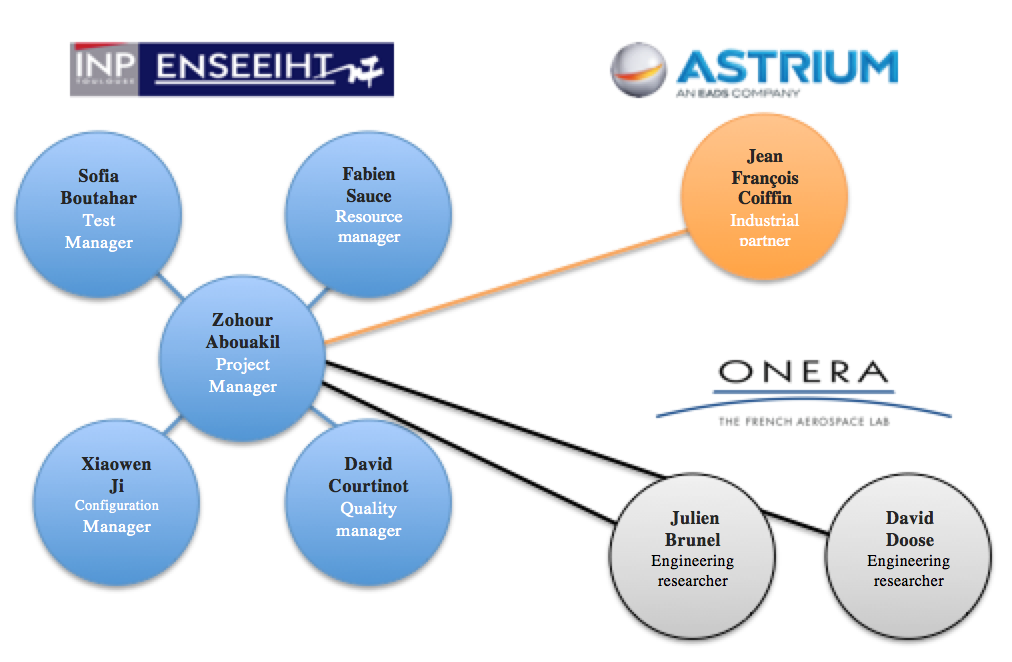
\includegraphics[scale=0.8]{data/teamOrganization.png}
~\\~\\Figure II.1 - The team organization of our project
\end{center}

\paragraph{}
\hspace{4mm}\textnormal{Although everybody was involved in the same manner in searching
, coding and testing stages, we gave everyone a role in
order to improve team organization. 
The project manager (Zohour \textsc{Abouakil}) has several responsabilities 
related to the project management. She is in charge of the
communication with the industrial coordinator, Mr. Jean Francois
\textsc{Coiffin} and the scheduling of the different appointments
. Fabien \textsc{Sauce} is in charge of the specifications and the documentation. 
Xiaowen is in charge of the version tool Git and takes care of all 
the software we use in the Project. Sofia \textsc{Boutahar} 
is responsible for the unitary tests and the regressions tests when 
there is a new version of the code or a part that is fully developped.}

\paragraph{}
\hspace{4mm}\textnormal{In addition to being the project manager,  Zohour establishes a 
contact with the client to see if the team is going in the right
direction or needs additional information.}

\section{Project objectives in terms of management and organization}

\paragraph{}
\hspace{4mm}\textnormal{\begin{itemize} 
\item Managing coordination of the partners and working groups 
engaged in project work.
\item Writing a detailed project planning including:
	\begin{itemize} 
	\item Developing and maintaining a detailed project
	 plan.
	\item Managing project deliverables in line with the 
	project plan.
	\item Recording and managing project issues and escalating where
	 necessary.
	\item Resolving issues and try to prevent them.
	\end{itemize}
\item Managing project scope and change control and escalating issues where necessary.
\item Monitoring project progress and performance.
\item Managing project evaluation and dissemination activities.
\item Final approval of the design specification.
\item Working closely with clients to ensure the project meets business needs.
\item Definition and management of the testing program.
\end{itemize}}

\section{Deliverable documents}

\subsection{Delivrable documents expected by ENSEEIHT and the industrial supervisor}

\vspace{3mm}
\begin{itemize}
\item Report in PDF format\vspace{1mm}
\item Development plan in PDF format\vspace{1mm}
\item Presentation supports\vspace{1mm}
\end{itemize}

\subsection{Delivrable documents expected by the client}

\vspace{3mm}
\begin{itemize}
\item Documented source code in Scala language\vspace{1mm}
\item Test strategy\vspace{1mm}
\item Architecture design document\vspace{1mm}
\end{itemize}

\section{Development plan}

\subsection{Development organization}

\paragraph{}
\hspace{4mm}\textnormal{We used the Scrum method, which is widely used, 
and recognized for its effectiveness. At first, 
we defined a product backlog containing all desired 
functionalities in the final product. In fact, this report is also a part 
of the product backlog. Next, we divided the project into three
 sprints (which means iterations). A sprint backlog is defined for 
each sprint, including all we need to realize at the end of an 
iteration. Each sprint lasts two weeks and lies in improve the 
software incrementally, so that it is close to product backlog. 
At the end of each sprint, we organised a meeting, in order to 
review the progress and propose improvements or modifications
 of planning, but in the process of a sprint, we cannot modify the 
sprint backlog. To finish, each day starts with a scrum meeting, on 
the meeting, each team member present his objective of the day
 and his actual difficulties.}

\subsection{Team organization approach}

\paragraph{}
\hspace{4mm}\textnormal{We will use an approach inspired by the XP (\textsc{extreme programming})
 method which is a practice of pair programming. Considering the amount of 
code that we will have to write,
 we find it unnecessary that the five team members work separately,
 and we consider as excellent to work in pairs, in order to prevent 
errors and bias of the program structure, so that we can save times
 in testing and debugging. As a consequence, four of us will work
 in pairs and the last one works individually or supervises us. The groups repartition 
may change as the tasks are completed.}

\subsection{Tasks organization}

\subsubsection{Task definition}

\paragraph{}
\hspace{4mm}\textnormal{The sprint backlog is a list of tasks that are identified by the members
 of the project and that has to be completed during the Scrum sprint.
During our meetings, we try to estimate how many hours and
development efforts needed to complete a task.
\\
\textbf{Sprint 1 backlog :}}

\vspace{3mm}
\begin{itemize}
\item AST parsing of procedure C++ code\vspace{1mm}
\item CFG conversion from parsed AST\vspace{1mm}
\item Model checking with simple properties\vspace{1mm}
\end{itemize}

\paragraph{}
\hspace{4mm}\textnormal{\textbf{Sprint 2 backlog :}}

\vspace{3mm}
\begin{itemize}
\item AST parsing of object oriented C++ code\vspace{1mm}
\item CFG conversion from parsed AST\vspace{1mm}
\item Model checking with simple criteria\vspace{1mm}
\end{itemize}

\paragraph{}
\hspace{4mm}\textnormal{\textbf{Sprint 3 backlog :}}

\vspace{3mm}
\begin{itemize}
\item Improved CFG conversion from parsed AST\vspace{1mm}
\item Model checking with complex criteria\vspace{1mm}
\end{itemize}

\subsubsection{Task planning}

\paragraph{}
\hspace{4mm}\textnormal{Our sprint backlog was maintained as a spreadsheet. 
During the Scrum sprint, each team member is requested to 
keep the sprint backlog updated.}

\section{Risk management}

\subsection{Risk management strategy}

\paragraph{}
\hspace{4mm}\textnormal{The first step in project risk management is to identify the risks
 that are present in the project. Also, some risks have a higher impact than others.
 Therefore, we spend our time on the risks that can cause the 
biggest losses and gains.}

\subsection{Risk analysis}


\paragraph{}
\hspace{4mm}\textnormal{Below a table that summarizes the major risks that we could face in our project and how we planned to prevent them.}

\begin{center}
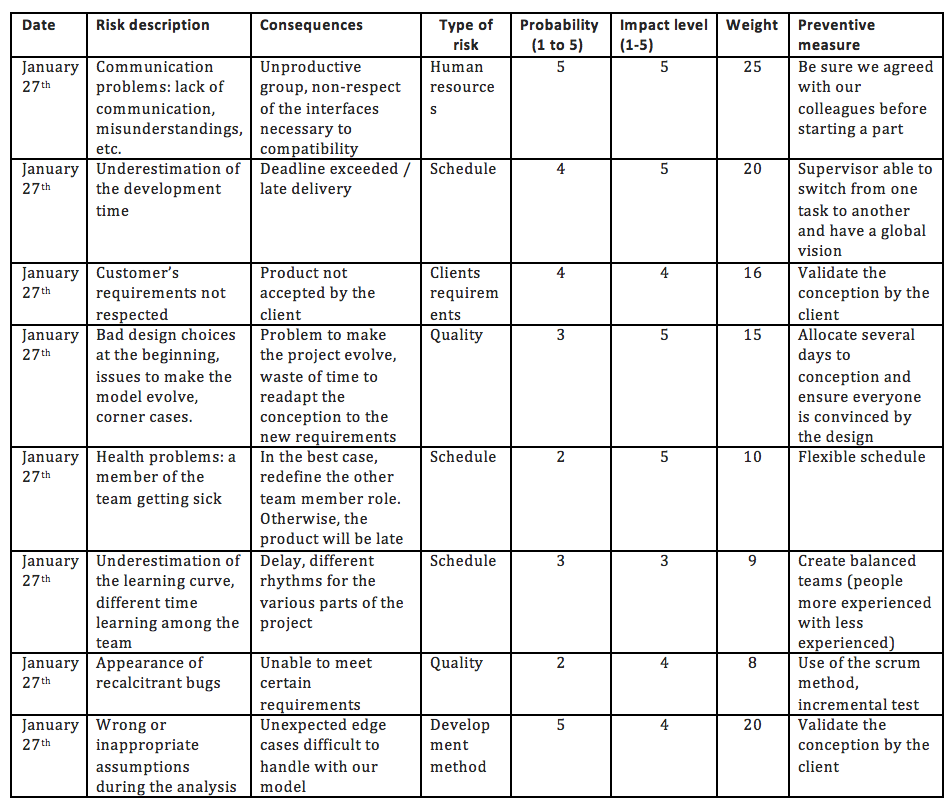
\includegraphics[scale=1.0]{data/RiskManagement.png}
~\\~\\Figure II.2 - The risk analysis for our project
\end{center}

\section{Resource management system}

\subsection{Versioning tool}

\paragraph{}
\hspace{4mm}\textnormal{We use Git to manage our project especially the versioning of the code
and the documents that we develop. Our choice was made 
because Git is a free and open source
 distributed version control system that handles any software 
project in a very efficient way. It also supports rapid branching and merging, 
and includes specific tools for visualizing and 
navigating through the development history.
All the delivrable documents are managed on a git repository, including documentation and reports. Anyone is allowed to commit at anytime, however any push must have been authorized by the quality responsible after the code has been thoroughly tested against a set of tests by the test responsible.}

\subsection{Communication between team members}

\paragraph{}
\hspace{4mm}\textnormal{We used Google Drive to share all the documents 
between the team members. Our drive was organized by folders: 
one with all the papers and the interesting documents
 that we found or we received from our clients,
one that contains all the documents that are related 
to the project management,
one with the notes that we take during the meetings either with 
the clients or the industrial coordinator,  
and the last one that contains all the useful links to have deeper
knowledge about the project's subject or the technologies used.}

\chapter{Code and documentation management}

\section{Quality checking}

\paragraph{}
\hspace{4mm}\textnormal{For ensuring that our coding rules are respected and
 evaluating the quality of our sources,
 we used a tool called Scalastyle that enables
, using an easy-to-use xml configuration file,
 to examine the scala code and indicates potential problems with it.
 Combined with a specific pulgin, this can be used to generate 
warnings or errors in the IDE the developer is using. 
Our settings are the following :}

\definecolor{mygray}{gray}{0.4}
\renewcommand{\arraystretch}{1.2}
\begin{center}
\begin{longtable}{|l|l|l|}
\hline
\textbf{\textcolor{mygray}{Rule}} & \textbf{\textcolor{mygray}{Description}} & \textbf{\textcolor{mygray}{Value}}  \\
\hline
FileLengthChecker & \small{Check the number of lines in a file} & 1500  \\
\hline
FileLineLengthChecker & \small{Check the number of characters in a line} & 140 \\
\hline
FileTabChecker & \small{Check that there are no tabs in a file} & enabled \\
\hline
ClassNamesChecker & \small{Check that class names match a regular}  & \^ [A-Z][A-a-z]*\$ \\
& \small{expression} & \\
\hline
\small{ClassTypeParameterChecker} & \small{Checks that type parameter to a class matches a} & \^[A-Z\_]\$ \\
& regular expression & \\
\hline
FileTabChecker & \small{Check that there are no tabs in a file} & enabled \\
\hline
\small{CyclomaticComplexityChecker} & \small{Checks that the cyclomatic complexity of a method} & 12 \\
&  \small{does exceed a value} & \\
\hline
EmptyClassChecker & \small{If a class/trait has no members, the braces are} & enabled \\
&  \small{unnecessary} & \\
\hline
\small{EqualsHashCodeChecker} & \small{Check that if a class implements either equals} & enabled \\ 
 & \small{or hashCode, it should implement the other} & \\
\hline
MethodLengthChecker & \small{Checks that methods do not exceed a maximum} & 50 \\
& \small{length} & \\
\hline
MethodNamesChecker & \small{Check that method names match a regular} & \^[a-z][A-Za-z0-9]*(\_=)?\$ \\
\tiny{.} & \small{expression} & \\
\hline
\small{MultipleStringLiteralsChecker} & \small{Checks that a string literal does not appear} & allowed = 2 \\
& \small{multiple times} & \\
\hline
\small{NotImplementedErrorUsage} & \small{Checks that the code does not have ??? operators} & enabled \\
\hline
NullChecker & \small{Check that null is not used} & enabled \\
\hline
\small{NumberOfMethodsInTypeChecker} & \small{Check that a class/trait/object does not have too} & maxMethods = 30 \\
& \small{many methods} & \\
\hline
NumberOfTypesChecker & \small{Checks that there are not too many types} & maxTypes = 20 \\
& \small{declared in a file} & \\
\hline
ObjectNamesChecker & \small{Check that object names match a regular}  & \^[A-Z][A-Za-z]*\$ \\
& \small{expression} & \\
\hline
ParameterNumberChecker & \small{Maximum number of parameters for a method} & maxParameters = 5 \\
\hline
RedundantIfChecker & \small{Checks that if expressions are not redundant, ie} & enabled \\
& \small{easily replaced by a variant of the condition} &  \\
\hline
ScalaDocChecker & \small{Checks that the ScalaDoc on documentable}  & enabled \\
& \small{members is well-formed} & \\
\hline
\end{longtable} 
\end{center}
\paragraph{}
\hspace{4mm}\textnormal{This project meets a need from our clients. 
Therefore our codes will probably be used, studied and modified. 
That is why we have set up this quality approach. 
All our codes should be understandable and well commented. 
To achieve that, our programs were constantly reviewed by our clients
as we gave them the link to our Git repository.}

\section{Verification and validation process}

\subsection{Verification process}

\paragraph{}
\hspace{4mm}\textnormal{Verification is the process in which we determine
whether the right solution is being developed.
Once a functionality of our product is completed, 
we analyze the results in order to
 verify that the requirements have been satisfied. 
 In addition, the verification is an ongoing process:
 at the each completion of each milestone, 
we performed a verification analysis to make 
sure we are still on track.}

\paragraph{}
\hspace{4mm}\textnormal{As we have chosen the \textsc{Extreme Programming} model for the programming 
aspect of the project, we considered that a code would have passed
 the quality test if at least the two members of a pair have checked 
it. This is up to the quality manager to ensure this has been done, 
otherwise he should do it himself. This is specific to the code quality 
checks and does not apply to the rest of the delivrable documents.}

\subsection{Validation process}

\paragraph{}
\hspace{4mm}\textnormal{Validation is the process in which we make sure that the solution
that we came up with is 
constructed correctly and according to the requirements 
and the specifications.
In this process, we performed various testing procedures on
 the code and tried to remove the defects as soon as possible. 
Once the found defects have being fixed, the process repeats itself.}

\paragraph{}
\hspace{4mm}\textnormal{}

\chapter{Technical aspects}

\section{Context}

\subsection{Motivations}

\paragraph{}
\hspace{4mm}\textnormal{Embedded systems and robotics are designed to interact with 
humans sometimes. Therefore, a single failure or a malfunction 
can really be catastrophic.  This is why various analyses are 
undertaken to limit and prevent such problems. Theses analysis aim
 to study the embedded code and prove that it does what it is 
supposed to do. The goal of our project is to find out whether the
 embedded code meets a number of programming rules by 
defining authorized and prohibited patterns. 
Our clients have an existing tool named Coccinelle that is 
developed at INRIA. This tool detects patterns and also offers
 the possibility to modify the code. However, this tool only works
 on C code.}

\subsection{Objectives}

\paragraph{}
\hspace{4mm}\textnormal{The model checking, which consists in asserting properties 
on a model thanks to graph search algorithms (for example),
 is one of those fields that can be applied to this matter.
 In this project, we are trying to build a model checker working
 on C++ code which takes the source code as an input and is 
transformed a few times in various abstract representations to end 
with a graph model that we are able to send to a model checker.}

\section{Definitions}

\subsection{The AST - \textsc{Abstract Syntax Tree}}

\paragraph{}
\hspace{4mm}\textnormal{The \textsc{AST} is an abstract (and low-level) representation of the 
abstract  syntactic structure of the source code.
It is a tree data-structure which describes the code in a purely 
syntactic point of view. Each node of the tree denotes a
 construct occurring in the source code. The syntax is "abstract" 
because it's not representing  every detail appearing in the real syntax. 
However, the \textsc{AST} can contain additional data as the position of 
an element in the source code node.
You can see below a
 simple \textsc{C/C++} code and its AST representation. 
The \textsc{AST} is provided by the Clang API, which performs the first step
 of our transformation chain.}

\begin{lstlisting}[language=java]
int main() {
    int a = 5;
    if (a > 6) {
        int c = 5;
        c *= 5;
    }
    int b = 17;
}
\end{lstlisting}
\begin{center}
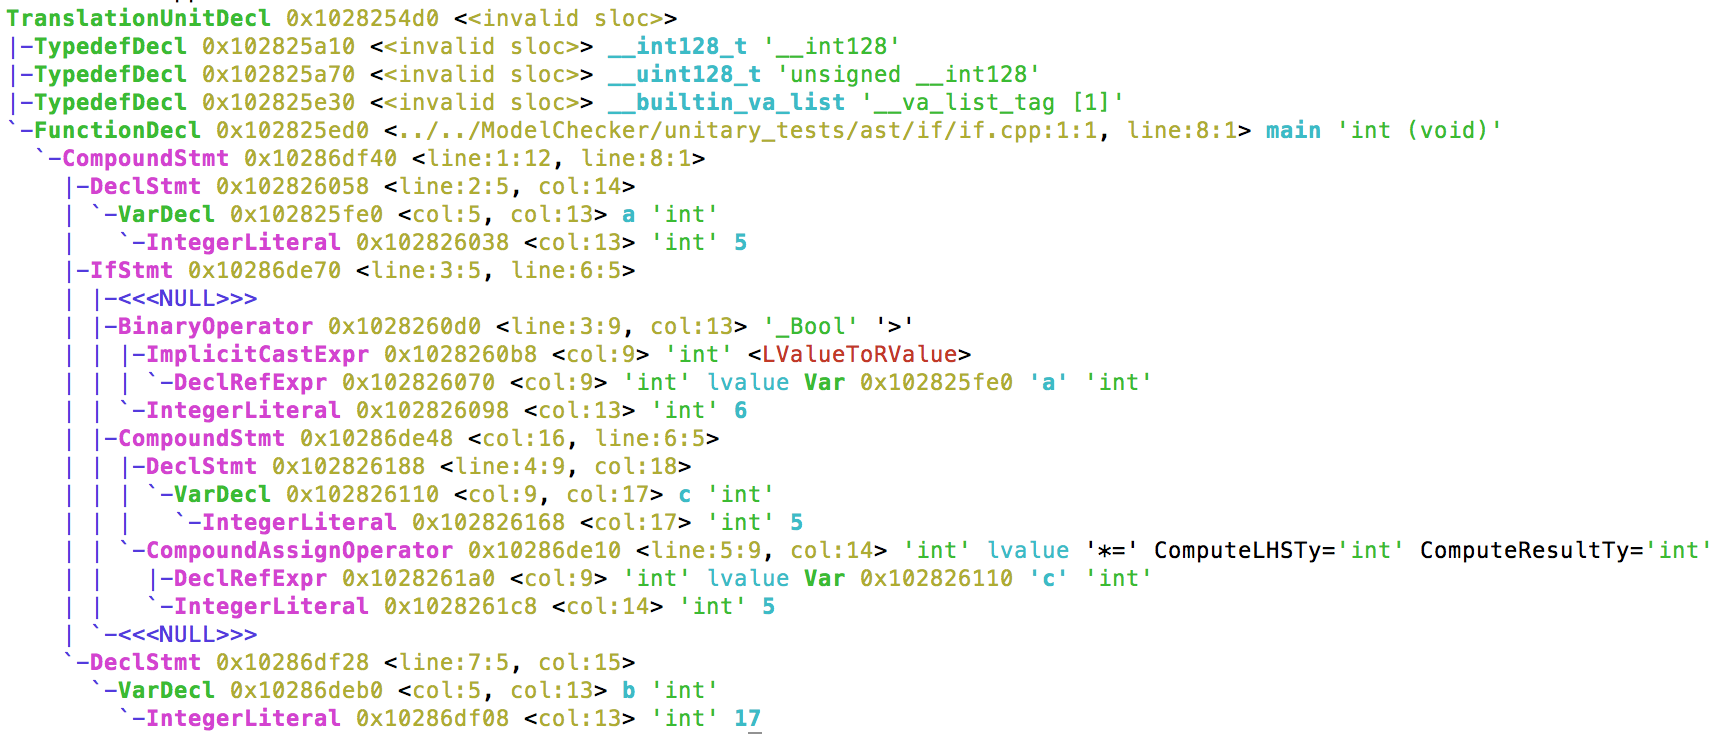
\includegraphics[scale=0.6]{data/ifClang.png}
~\\~\\Figure IV.1 - The AST of the C++ code generated by the clang API
\end{center}

\paragraph{}
\hspace{4mm}\textnormal{\definecolor{oliveGreen}{RGB}{0,102,0}
The indentation in the AST is the depth of a node. Nodes that have
the same level of indentation are brothers. Each node can have 
children that are separated by a new line and a \textcolor{blue}{|\_}. We should notice
that the last child of a node starts it's representative line by \textcolor{blue}{`\_}
. For example the \textcolor{oliveGreen}{TranslationUnitDecl} has four children :
the first three childs are \textcolor{oliveGreen}{TypedefDef} and the last one is a \textcolor{oliveGreen}{FunctionDecl}.
The toplevel declaration in a translation unit is always the
 translation unit declaration. 
In this example, our first user written declaration 
is the declaration of the function "main" that contains
a declaration of the variable a and then an If statement.
The \textcolor{magenta}{IfStmt} (if statement) has a condition and a body. The condition is 
described in this example by the binary operator \textcolor{blue}{>} that has two
childs which are the operands \textcolor{blue}{a} and \textcolor{blue}{6}. 
The body of the \textcolor{magenta}{IfStmt} is described by the compound statement which is 
a combination of two or more simple statements. In this case, it's 
a combination of a \textcolor{magenta}{declStmt} (declaration statement) in which the declaration and 
initialization of  the variable \textcolor{blue}{c} to \textcolor{blue}{5} 
is described and a compoundAssignOperator 
in which the assignment operation is described.
In the end, there is a \textcolor{magenta}{DeclStmt} that describes the declaration and initialization
of the variable \textcolor{blue}{b} to \textcolor{blue}{17}.}

\end{document}
